\documentclass[a4paper,12pt]{article}
\usepackage{mathptmx}
\usepackage{enumitem} 
\usepackage{geometry}
\usepackage{amsmath}
\usepackage{setspace}
\usepackage{graphicx}
\usepackage{caption}
\usepackage{float}
\usepackage{amsfonts}
\usepackage{amssymb}
\usepackage{hyperref}
\usepackage{listings}
\usepackage{color}
\usepackage[utf8]{inputenc}  
\usepackage{cite}  
\usepackage{booktabs}

\geometry{margin=1in}

\begin{document}

\begin{titlepage}
    \centering
    
\includegraphics[width=8cm]{Images/Nanyang_Technological_University-Logo.wine.png}\par\vspace{1cm}
    {\scshape\LARGE Nanyang Technological University \par}
    \vspace{1.5cm}
    {\huge\bfseries EE6407 Genetic Algorithms \& Machine Learning\par}
    \vspace{0.5cm}
    {\Large Assignment 1 \& 2 Report\par}
    \vspace{2cm}
    {\large MSc in Electrical and Electronic Engineering\par}
    {\large Yan Ziming\par}
    {\large G2507084J\par}
    \vfill
    {\large \today \par}
\end{titlepage}

\newpage
\tableofcontents
\newpage

\section{Introduction}

\section{Assignment 1}
\subsection{Handling Missing Values and Outliers}

\subsubsection{Missing values}
\textbf{\textit{Detection:}}\\
\textbf{\textit{Handling:}}
\subsubsection{Outliers}
\textbf{\textit{Detection:}}\\
\textbf{\textit{Handling:}}

\subsection{Design a Naïve Bayes classifier}
\begin{figure}[h]
    \centering
    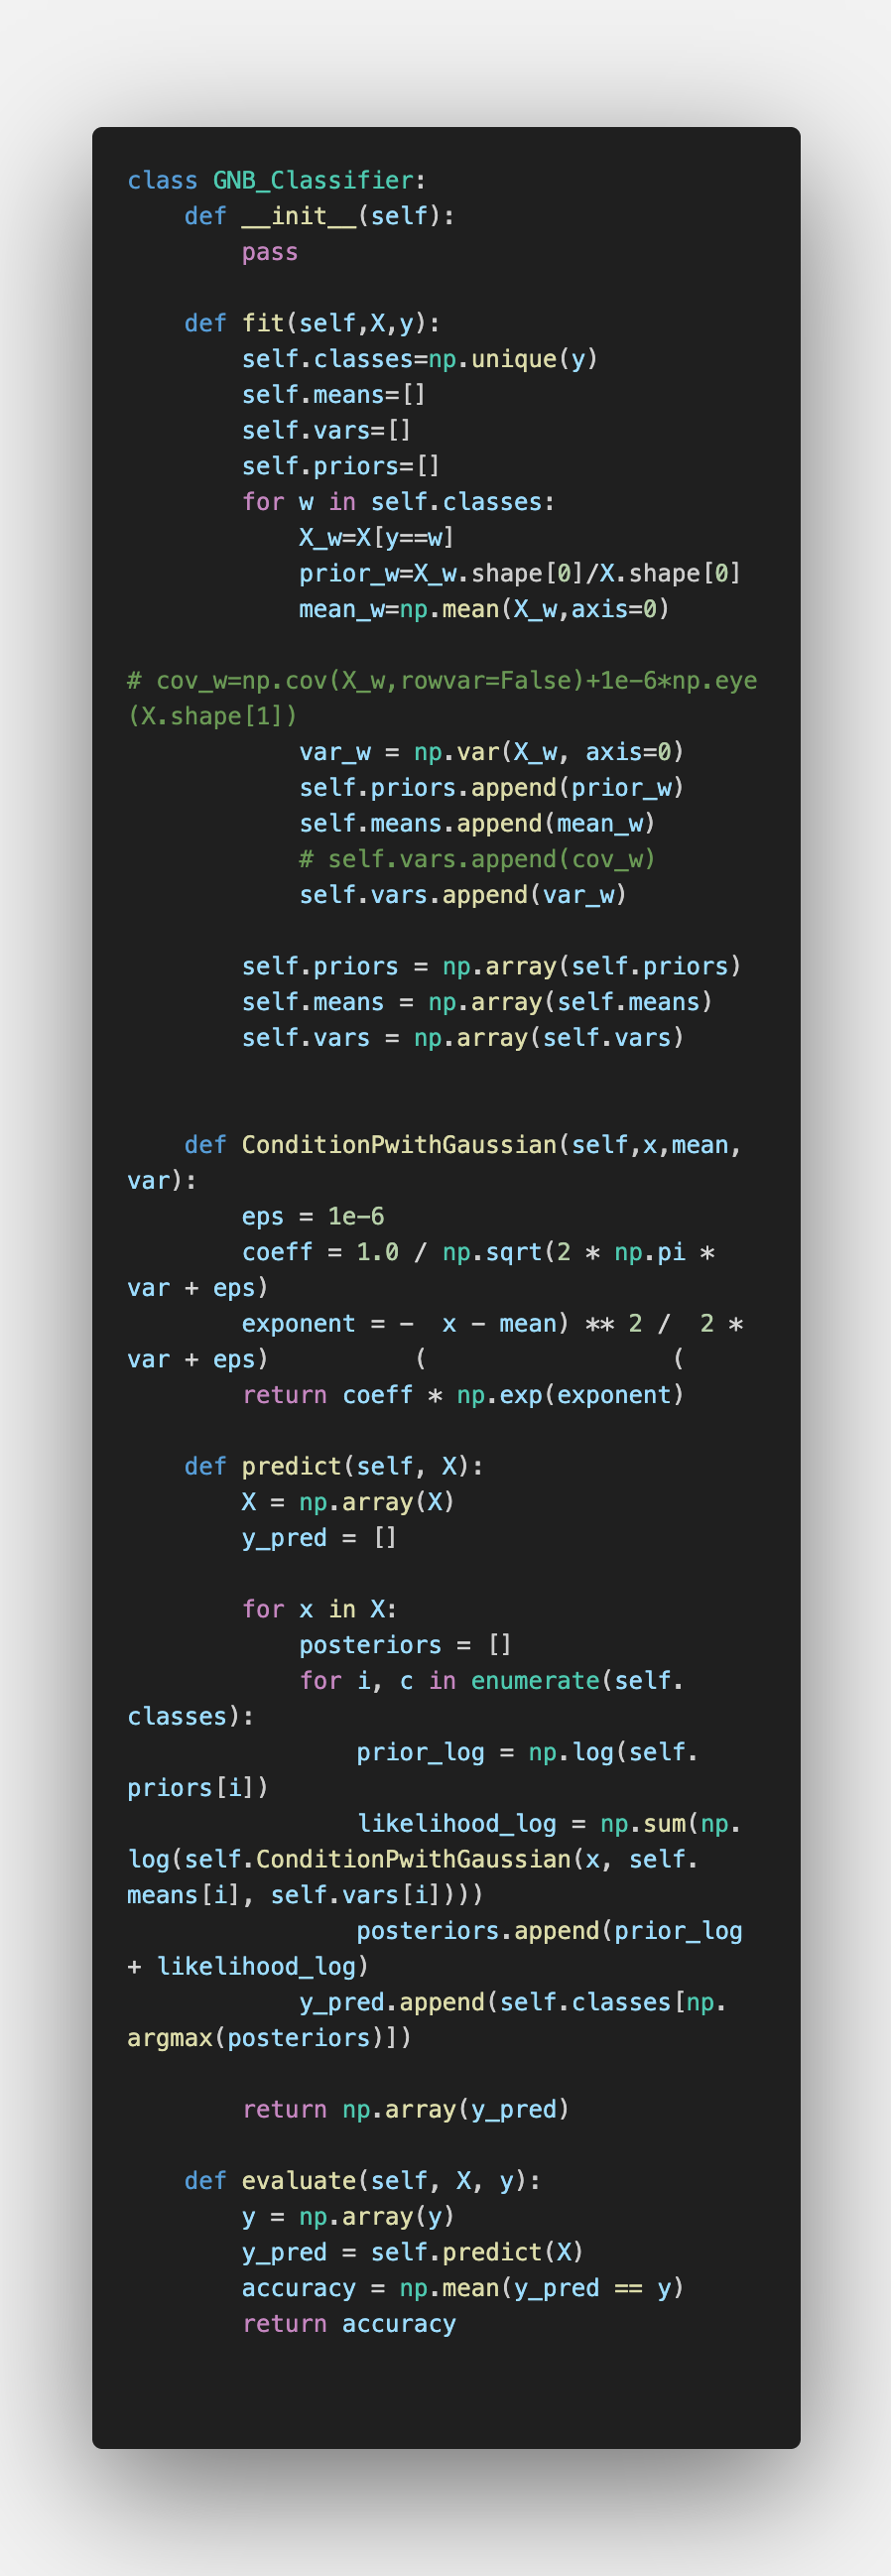
\includegraphics[width=\textwidth]{Images/Assignment_1/gnb_classifier_code.png}
    \caption{Code of Classifier Establishment}
    \label{fig:code_cell_0}
\end{figure}
\subsection{Prediction and Analysis}
\begin{table}[H]
\centering
\caption{Results of Gaussian Naive Bayes Classifier}
\begin{tabular}{ll}
\toprule
Metric & Value \\
\midrule
Training Accuracy & 0.958333 \\
Predicted Labels & [1 1 1 1 1 1 1 1 1 1 3 2 2 2 2 2 2 2 2 2 2 3 3 3 3 3 3 3 3 3] \\
\bottomrule
\end{tabular}
\end{table}


\section{Assignment 2}

\section{Conclusion}
\end{document}